%\documentclass[12pt,compress,aspectratio=169]{beamer}
%\input{../mybeamer}
%
\chapter{Electromagnetic Waves}
\label{chapter:lightwaves}

\section{Electromagnetic Wave}
%
%
%\begin{frame}{New Physics: Maxwell's Equations}

%    \centering
%    \pic1{PORTRAIT-James-Clerk-Maxwell}\\
%    James Clerk Maxwell
%    
%    \begin{itemize}
%    \item Classical laws of electrodynamics
%    \item Published in 1861 and 1862
%    \item Explains the relationship between
%      \begin{itemize}
%      \item Electricity
%      \item Electric Circuits
%      \item Magnetism
%      \item Optics
%      \end{itemize}
%    \item Previously these disciplines are thought to be separate and not
%      related
%    \end{itemize}


\subsection{Maxwell's Equations}

\begin{align}
  \nabla\cdot\vec E &=\frac\rho{\varepsilon_0}\label{eq:gauss-electricity}\\
  \nabla\cdot\vec B &= 0\label{eq:gauss-magnetism}\\
  \nabla\times\vec E &=-\frac{\partial\vec B}{\partial t}
  \label{eq:faradays-law-2}\\
  \nabla\times\vec B &=
  -\mu_0\vec J+\mu_0\varepsilon_0\frac{\partial\vec E}{\partial t}
  \label{eq:amperes-law}
\end{align}

That's a lot of symbols that you won't recognize. Solving them require a lot of
difficult calculus that even most science students in university don't need to
learn.\footnote{i.e.\ you don't need to learn this!}
\begin{itemize}[itemsep=6pt]
\item\textbf{Gauss's law for electricity:} Electric fields must begin and/or
  end at a charge.
\item\textbf{Gauss's law for magnetism:} Magnetic field lines do not have a
  beginning or an end.
\item\textbf{Faraday's law:} Fluctuations in the magnetic field in time
  produces an electric field that varies in space.
\item\textbf{Ampere's law:} Fluctuations in the electric field in time produces
  a magnetic field that varies in space.
\end{itemize}


\subsection{Speed of Light}

Disturbances in the electric and magnetic fields propagate in a vacuum as an
\textbf{electromagnetic wave} with defined speed that we now call
\textbf{speed of light}):
\begin{equation}
  \boxed{
    c_0=\frac1{\sqrt{\varepsilon_0\mu_0}}=\SI{299792458}{\meter\per\second}
  }
\end{equation}
The speed of light is based on two constants that we have studied earlier in
electricity and magnetism:
\begin{itemize}
\item\textbf{Permittivity of free space} $\varepsilon_0$: the ability of a
  vacuum to resist the formation of an electric field within it. This constant
  is related to the Coulomb constant.
\item\textbf{Permeability of free space} $\mu_0$: A measure of the ability
  of a vacuum to become magnetized.
\end{itemize}
By 1862, the speed of light was already measured to within about
\SI{.6}{\percent} of this value (By french physicist L\'{e}on Foucault using a
rotating mirror experiment. His experimental value was \num{298000}$\pm 500$
\si{\metre\per\second}). So Maxwell's equations show that light is (probably)
an electromagnetic wave.


%{The Electromagnetic Spectrum}
\begin{figure}[ht]
  \centering
  \pic{.8}{lightWaves2/graphics/electromagneticspectrum-141b490bac872789434}
\end{figure}



\section{Polarization of Light} %{Combining Everything We Know}

%  \begin{itemize}
%  \item Light is an electromagnetic wave, generated by
%    \begin{itemize}
%    \item An oscillating charged particle (e.g. shaking an electron violently)
%    \item An alternating (``A/C'') current (i.e.\ many oscillating charges)
%    \item Through black-body radiation
%    \end{itemize}
%  \item EM waves have both an oscillating electric field ($\vec E$) and
%    magnetic field ($\vec B$), because
%    \begin{itemize}
%    \item A charged particle creates an electric field, and
%    \item A moving charged particle creates a magnetic field
%    \end{itemize}
%  \item $\vec E$ and $\vec B$ are always perpendicular to one another,
%    according to Maxwell's equations
%  \end{itemize}

%
%
%
%%{On Polarization of Light}
%%  Charged particles can vibrate in any direction, so the oscillating $\vec E$
%%  and $\vec B$ can look quite chaotic. We can only guarantee that, $\vec E$ and
%%  $\vec B$ are:
%%  \begin{itemize}
%%  \item Always perpendicular to each other
%%  \item Always perpendicular to the direction of wave travel
%%  \item This kind of light (or general EM wave) is ``unpolarized''
%%  \item Most EM waves you experience in life are this kind:
%%  \end{itemize}
%%  \begin{center}
%%    \vspace{-.1in}\pic{.7}{graphics/T1Zlt}
%%  \end{center}
%
%
%
%
%%{On Polarization of Light}
%%  But if we can confine $\vec E$ and $\vec B$ to one plane, then we have a
%%  ``polarized'' light:
%%  \begin{center}
%%    \pic{.4}{graphics/em-20field}
%%  \end{center}
%%  There are a few ways to do this\ldots
%
%%
%%
%%
%%{On Polarization of Light}{Using Polarizer}
%%  \begin{itemize}
%%  \item A polarizer is really just a grill that only lets in vibration in one
%%    direction through:
%%    \begin{center}
%%      \pic{.4}{graphics/polarizerfencemodel600}
%%    \end{center}
%%  \item The incoming wave can be vibrating in any direction, but outgoing wave
%%    only vibrates in one direction.
%%  \item Sunglasses with polarizing lens
%%  \item Polarizer filters on cameras
%%  \end{itemize}
%
%%
%%
%%
%%{Polarization by Reflection}
%
%%    \pic1{graphics/01fig16}
%%    
%%    At \textbf{Brewster's angle}, the light reflected off a medium (e.g.\
%%    glass, water) is also polarized
%%
%%    \eq{-.1in}{
%%      \theta_B =\tan^{-1}\left(\frac{n_2}{n_1}\right)
%%    }
%%    \begin{itemize}
%%    \item Incident light is non-polarized
%%    \item Reflected light is polarized
%%    \item Refracted light is partially polarized
%%    \item For water ($n=1.33$), $\theta_B=\ang{53}$
%%    \item For glass ($n=1.5$), $\theta_B=\ang{56}$
%%    \end{itemize}
%
%
%
%
\section{Reflection and Refraction}
%
%{Reflection and Refraction}
%  We begin with a model of a beam of light traveling towards an interface
%  between two ``indexed material'':
%  \begin{center}
%    \begin{tikzpicture}[scale=.8,very thick]
%      \fill[gray!50] (-3,-2) rectangle (3,0);
%      \draw[thick] (-3,0)--(3,0);
%      \begin{scope}[rotate=45,red]
%        \draw[vectors] (0,2.5)--(0,1);
%        \draw[very thick] (0,2)--(0,0);
%        \draw[very thick] (0,0)--(2.5,0) node[right]{Reflection};
%        \draw[vectors] (0,0)--(1.75,0);
%      \end{scope}
%      \draw[rotate=30,red] (0,0)--(0,-2.3)
%      node[above right]{Refraction};
%      \draw[rotate=30,->,red] (0,0)--(0,-1);
%      \draw[dashed,black!70,thick] (0,2)--(0,-2);
%      \draw[axes] (0,1.5) arc (90:135:1.5) node[midway,above]{$\theta_1$};
%      \draw[axes] (0,1.2) arc (90:45:1.2) node[midway,above]{$\theta_r$};
%      \draw[axes] (0,-1.5) arc (270:300:1.5) node[pos=0,left]{$\theta_2$};
%      \node[above] at (-2.2,0){$n_1$};
%      \node[below] at (-2.2,0){$n_2$};
%      \node[above] at (2.2,0){$v_1$};
%      \node[below] at (2.2,0){$v_2$};
%    \end{tikzpicture}
%  \end{center}
The \textbf{index of refraction} (or \textbf{refractive index}, or just
\textbf{index}) of the two media is defined as the ratio of speeds of light in
a vacuum $c_0$ and in the medium $c$:
\begin{equation}
  n=\frac{c_0}c\geq 1
\end{equation}

%
%
%
%{Reflection of Light}
In the \textbf{law of reflection}, the incident ray, the reflected ray, and the
normal to the surface of the mirror all lie in the same plane, and the angle of
reflection $\theta_r$ is equal to the angle of incidence $\theta_1$:
\begin{equation}
  \boxed{\theta_r=\theta_1}
\end{equation}
%  
%  \begin{center}
%    \vspace{-.2in}
%    \pic{.6}{graphics/Types-of-reflection}
%  \end{center}

%
%
%
%{Specular Reflection Example}
%  \begin{center}
%    \pic{.55}{graphics/Lake-reflection}
%  \end{center}
%  This photo of Lake Matheson shows specular reflection in the water of the
%  lake with reflected images of Aoraki/Mt Cook (left) and Mt Tasman (right).
%  The very still lake water provides a perfectly smooth surface for this to
%  occur.

%
%
%
%%{Intensity of Reflected Light}
%%  When the incident and reflected angles normal, i.e.
%%  $\theta_1=\theta_r=0$, the reflected intensity of light $I$ is related to the
%%  incident intensity $I_0$ by the indices of the two material ($n_1$ and $n_2$):
%%
%\begin{equation}
%%    I=\left[\frac{n_1-n_2}{n_1+n_2}\right]^2 I_0
%\end{equation}
%%  
%%  The intensity of a wave is the power $P$ over the area $A$ that the wave
%%  passes through:
%%
%\begin{equation}
%%    I=\frac PA
%\end{equation}
%%
%%  The reflected intensity is lower than the incident, indicating that some of
%%  the energy from the incident wave is transmitted into the second medium.
%
%
%
%
\section{Refraction}

\textbf{Refraction} occurs when light is transmitted from one medium to another
at an oblique angle. The wave changes direction due to the difference in the
speed of light in the two media.
%  \begin{center}
%    \begin{tikzpicture}[scale=.9]
%      \fill[thick,gray!30] (-3,-2) rectangle (3,0);
%      \draw[thick] (-3,0)--(3,0);
%      \draw[red,very thick] (-2,2)--(0,0)--(1,-2);
%      \draw[thick,dashed] (0,2)--(0,-2);
%      \draw[axes] (0,1) arc (90:135:1) node[midway,above]{$\theta_1$};
%      \draw[axes] (0,-1) arc (270:297:1) node[midway,below]{$\theta_2$};
%      \node[above] at (-2,0){$n_1$};
%      \node[below] at (-2,0){$n_2$};
%      \node[above] at (2,0){$v_1$};
%      \node[below] at (2,0){$v_2$};
%    \end{tikzpicture}
%  \end{center}

\textbf{Snell's law} (or \textbf{law of refraction}) relates the refractive
indices $n$ of the two media to the directions of propagation in terms of the
angles $\theta$ to the normal.
\begin{equation}
  \boxed{n_1\sin\theta_1=n_2\sin\theta_2}
\end{equation}
This equation holds for the refraction of any kind of wave incident on a
boundary surface separating two media (e.g.\ surface ocean wave at two depths)

%
%
%
%%{Refraction and Huygens Principle}
%
%%    \pic{1}{graphics/huygen}
%%    
%%    We can explain the refraction phenomenon using Huygens' Principle
%
%
%
%
%
%
%{Index of Refraction}
When light enters a new medium, the \emph{frequency} remains the same: the
atoms in the new medium would absorb and then radiate the light at the same
frequency. However, the \emph{speed} of the radiated wave is different,
therefore a different \emph{wavelength} is observed: 
\begin{equation}
  \boxed{\frac{n_1}{n_2}=\frac{\lambda_2}{\lambda_1}}
\end{equation}
You can work this out using the relationship between wave speed, frequency
and wavelength: $c=f\lambda$

\begin{table}[ht]
  \centering
  \begin{tabular}{c|c||c|c}
    \rowcolor{pink}
    \textbf{Material} & $n$ & \textbf{Material} & $n$\\ \hline
    Vacuum           & 1        & Ethanol     & 1.362 \\
    Air              & 1.000277 & Glycerine   & 1.473 \\
    Water at \SI{20}\celsius & 1.33 & Ice  & 1.31 \\
    Carbon disulfide & 1.63     & Polystyrene & 1.59 \\
    Methylene iodide & 1.74     & Crown glass & 1.50-1.62\\
    Diamond          & 2.417    & Flint glass & 1.57-1.75\\
  \end{tabular}
  \caption{Index of refraction of common materials}
\end{table}
The values given are \emph{approximate} and do not account for the small
variation of index with light wavelength. That's called \textbf{dispersion}.


\subsection{Total Internal Reflection}
When light is transmitted from a high index material to a lower index material
(i.e.\ $n_1>n_2$), Snell's law (Eq.~\ref{eq:law-of-refraction}) shows that the
angle of refraction $\theta_2$ is greater than the angle of incident $\theta_1$
(i.e.\ $\theta_2>\theta_1$), as shown in Figure~\ref{fig:no-tir}.

\begin{figure}[ht]
  \centering
  \begin{subfigure}[t]{.32\linewidth}
    \centering
    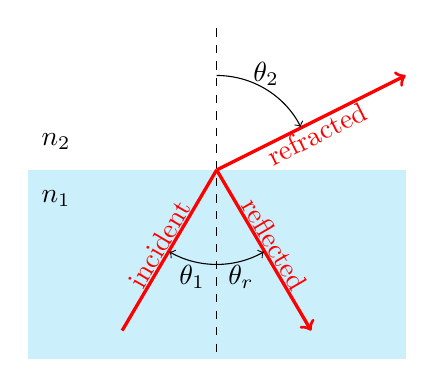
\begin{tikzpicture}[scale=1.2]
      \fill[color=cyan!20] rectangle (4,-2);
      \node at (.3,-.3) {$n_1$};
      \node at (.3,.3) {$n_2$};
      \draw[dashed] (2,1.5)--(2,-2);
      \begin{scope}[very thick,red]
        \draw (1,-1.7)--(2,0) node[sloped,midway,above=-3]{incident};
        \draw[->] (2,0)--(3,-1.7) node[sloped,midway,above=-3]{reflected};
        \draw[->] (2,0)--(4,1) node[sloped,midway,below=-3]{refracted};
      \end{scope}
      \draw[->] (2,-1) arc (270:240:1) node[midway,below=-2]{$\theta_1$};
      \draw[->] (2,-1) arc (270:300:1) node[midway,below=-2]{$\theta_r$};
      \draw[->] (2,1) arc (90:27:1) node[midway,above=-2]{$\theta_2$};
    \end{tikzpicture}
    \caption{Light transmits from high to low index material at small angle.}
    \label{fig:no-tir}
  \end{subfigure}
  \hspace{\stretch1}
  \begin{subfigure}[t]{.32\linewidth}
    \centering
    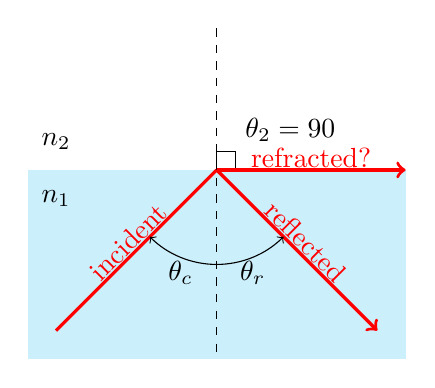
\begin{tikzpicture}[scale=1.2]
      \fill[color=cyan!20] rectangle (4,-2);
      \node at (.3,-.3) {$n_1$};
      \node at (.3,.3) {$n_2$};
      \draw[dashed] (2,1.5)--(2,-2);
      \draw (2,0) rectangle +(.2,.2) node[above right]{$\theta_2=\ang{90}$};
      \begin{scope}[very thick,red]
        \draw (.3,-1.7)--(2,0) node[sloped,midway,above=-3]{incident};
        \draw[->] (2,0)--(4,0) node[midway,above=-3]{refracted?};
        \draw[->] (2,0)--(3.7,-1.7) node[sloped,midway,above=-3]{reflected};
      \end{scope}
      \draw[->] (2,-1) arc (270:225:1) node[midway,below=-2]{$\theta_c$};
      \draw[->] (2,-1) arc (270:315:1) node[midway,below=-2]{$\theta_r$};
    \end{tikzpicture}
    \caption{At critical angle $\theta_1=\theta_c$, angle of refraction is
      \ang{90}}
    \label{fig:critical-angle}
  \end{subfigure}
  \hspace{\stretch1}
  \begin{subfigure}[t]{.32\linewidth}
    \centering
    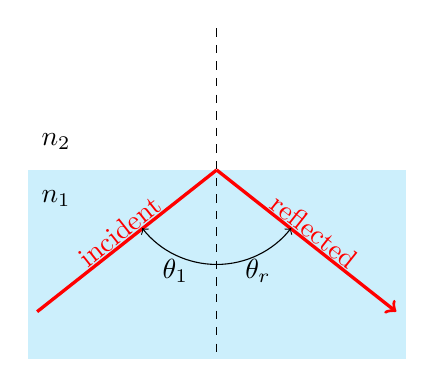
\begin{tikzpicture}[scale=1.2]
      \fill[color=cyan!20] rectangle (4,-2);
      \node at (.3,-.3) {$n_1$};
      \node at (.3,.3) {$n_2$};
      \draw[dashed] (2,1.5)--(2,-2);
      \begin{scope}[very thick,red]    
        \draw (.1,-1.5)--(2,0) node[sloped,midway,above=-3]{incident};
        \draw[->] (2,0)--(3.9,-1.5) node[sloped,midway,above=-3]{reflected};
      \end{scope}
      \draw[->] (2,-1) arc (270:218:1) node[midway,below=-2]{$\theta_1$};
      \draw[->] (2,-1) arc (270:322:1) node[midway,below=-2]{$\theta_r$};
    \end{tikzpicture}
    \caption{Beyond the critical angle, all light is reflected back}
    \label{fig:TIR}
  \end{subfigure}
\end{figure}
As the angle of incident increases, the angle of refraction will reach \ang{90}
first. When the angle of refraction is at \ang{90}, the angle of incident is
called the \textbf{critical angle} $\theta_c$, as shown in
Figure~\ref{fig:critical-angle}. Refracted light can still be observed
\emph{at} the interface, but only if the interface is perfectly smooth. We can
calculate the critical angle by setting $\theta_2=\ang{90}$ (i.e.\
$\sin\theta_2=1$) and solving for $\theta_1$:
\begin{equation}
  \boxed{
    \theta_c=\sin^{-1}\left(\frac{n_2}{n_1}\right)
  }
\end{equation}
Critical angle $\theta_c$ for water-air interface ($n_\text{air}=1$ and
$n_\text{water}=1.33$) is \ang{48.6}.

When the angle of incident is greater than the critical angle (i.e.\
$\theta_1>\theta_c$), Snell's law fails, because $\sin\theta_2$ cannot be
greater than 1. At this time, \textbf{total internal reflection} occurs. All
the incident light onto the interface is reflected back into the first medium,
as shown in Figure~\ref{fig:TIR}. Obviously, total internal reflection can only
occur when light travels from high index material towards a lower index
material, $n_1>n_2$.



\section{Dispersion of Light}
%%{Color of Light and Wavelength}
%%  Human eyes perceive different frequencies of light as different colors. The
%%  visible spectrum of light range from about \SI{380}{\nano\metre} (violet) to
%%  about \SI{700}{\nano\metre} (red).
%%  \begin{center}
%%    \pic{.6}{graphics/electromagneticspectrum-141b490bac872789434}
%%  \end{center}
%%  A good question to ask: where is \emph{purple}?
%



The index of refraction of a material varies slightly with wavelength
$\lambda$. This is called \textbf{dispersion}. The dispersion of light through
a prism is why we can see the rainbow colors from a beam of white light:
%  \begin{center}
%    \pic{.3}{graphics/Prism_rainbow_schema}
%  \end{center}
The index of refraction for shorter wavelengths is always higher than for
longer wavelengths.

\begin{itemize}
\item\textbf{White light} is a light that is composed of multiple colours
  in the visible-light spectrum
\item When white light passes through a prism it is separated into
  different colours
\item This is because the refractive index $n$ varies slightly with
  wavelengths (without this variation, we'd never see a rainbow)
\item The phenomenon is of splitting light into its component colours is
  called \textbf{dispersion}
\end{itemize}
%
%
%{Wavelength Dependency of Index of Refraction}
%  We can see that for different kinds of glass, the index of refraction can vary
%  significantly through the visible spectrum.
%  \begin{center}
%    \pic{.45}{graphics/Dispersion-curve}
%  \end{center}



\subsection{Chromatic Aberration}
The reason that chromatic aberration happens is the same reason that prisms
work: through dispersion of light
%  \begin{center}
%    \pic{.4}{graphics/chromatic-aberration-feature-image}
%  \end{center}
The focal lengths for different frequencies (colour) of light are different,
thus blurring the image. So how do we fix it?

By arranging different lenses of different materials and geometries, we can
correct for the chromatic aberration.
%  \begin{center}
%    \pic{.4}{graphics/Apochromatic-Lens}
%  \end{center}
Lens design is a closely guarded secret by camera companies. Shape of the
lens, material and coating are all factors. A ``lens'' on a DSLR camera can
have up to 30 lens ``elements''






\chapter{Geometric Optics}
\label{chapter:geom-optics}


\section{Mirrors: Image Forming by Reflection}
%
%{Spherical Mirror}

%    We can imagine a \textbf{spherical mirror} to be a sphere with smooth
%    light-reflecting surfaces inside and out.
%    \begin{itemize}
%    \item A \textbf{concave mirror} is the surface \emph{inside} the spherical
%      mirror
%    \item A \textbf{convex mirror} is the surface \emph{outside} the spherical
%      mirror
%    \end{itemize}

%    \pic{1}{graphics/spherical-mirror}


%
%
%
%{Spherical Mirror}
%  The cross-section diagram of the mirror:
%  \begin{center}
%    \begin{tikzpicture}[scale=.9,thick]
%      \draw[magenta] (3,0)--(-3,0) node[left]{PA};
%      \draw (3,0) arc (0: 30:3);
%      \draw (3,0) arc (0:-30:3) node[below]{mirror};
%      \fill circle (.05) node[below]{$C$};
%      \fill (3,0) circle (.05) node[right]{$V$};
%      \draw[rotate=20,axes] (0,0)--(3,0) node[midway,above]{$R$};
%    \end{tikzpicture}
%  \end{center}
%  \begin{itemize}
%  \item\textbf{Center of curvature} $C$: centre of the imaginary sphere
%    with the same radius as the mirror
%  \item\textbf{Radius of curvature} $R$ is any straight line from the
%    centre of curvature to the curved surface
%  \item\textbf{Vertex} $V$ is the geometric centre of the mirror surface
%  \item\textbf{Principal axis} ``PA'': a straight that passes through $V$ and
%    $C$
%  \end{itemize}

%
%
%{Spherical vs.\ Parabolic Mirror}
%  \begin{itemize}
%  \item Rays that are closed to the PA are called \textbf{paraxial rays}; they
%    converge at a single point called the \textbf{focal point} $F$
%  \item Rays that are far away from the PA are called \textbf{nonparaxial rays};
%    they converge to different points
%  \end{itemize}
%  \begin{center}
%    \pic{.6}{graphics/spherical-vs-parabolic}
%  \end{center}
%  In order for all beams of light to converge to the focal point, a
%  \textbf{parabolic mirror} must be used instead of a spherical mirror.

%
%
%
%{Focal Point and Focal Length}
The focal point $F$ is exactly half way between the centre of curvature and
the mirror, and the distance to the mirror is called the \textbf{focal length}
$f$:
\begin{equation}
  \boxed{f=\frac12 r}
\end{equation}
%  \begin{center}
%    \begin{tikzpicture}[thick]
%      \draw[magenta,dashed] (3,0)--(-3,0) node[left]{PA};
%      \draw (3,0) arc (0: 30:3);
%      \draw (3,0) arc (0:-30:3) node[below]{mirror};
%      \fill circle (.05) node[below]{$C$};
%      \fill (3,0) circle (.05) node[right]{$V$};
%      \fill[blue] (1.5,0) circle (.05) node[below]{$F$};
%      \draw[blue,<->,very thick] (1.5,0)--(3,0) node[midway,below]{$f$};
%      \draw[axes,rotate=20] (0,0)--(3,0) node[midway,above]{$R$};
%    \end{tikzpicture}
%  \end{center}  

%
%
%
%{Mirror Equation}
In terms of the focal length, the \textbf{mirror equation} is expressed as
\begin{equation}
  \boxed{\frac1s+\frac1{s'}=\frac1f}
\end{equation}
%  \begin{center}
%    \begin{tabular}{l|c|c}
%      \rowcolor{pink}
%      \textbf{Quantity} & \textbf{Symbol} & \textbf{SI Unit} \\ \hline
%      Distance to object & $s$  & \si\metre \\
%      Distance to image  & $s'$ & \si\metre \\
%      Focal length       & $f$  & \si\metre 
%    \end{tabular}
%  \end{center}
This equation is derived mathematically using basic geometry and the
small-angle approximation.

%
%
%
%{Sign Convention for the Mirror Equation}
When working with the mirror equation, we use the following sign convention:  
%\begin{equation}
%  \boxed{\frac1s+\frac1{s'}=\frac1f}
%\end{equation}
\begin{center}
  \begin{tabular}{ccl}
    \hline
    $s$ & $+$ & object is in front of the mirror (real object) \\
    & $-$ & object is behind the mirror (virtual object)\\\hline
    $s'$ & $+$ & image is in front of the mirror (real image)\\
    & $-$ & image is in behind the mirror (virtual image)\\\hline
    $R$, $f$ & $+$ & centre of curvature is in front of the mirror
    (concave mirror)\\
    & $-$ & centre of curvature is behind the mirror (convex mirror)\\
    \hline
  \end{tabular}
\end{center}

%
%
%
%{Lateral Magnification}
Using the sign convention as the mirror equation, the
\textbf{lateral magnification} of the object is given by:
\begin{equation}
  \boxed{m=\frac{h'}h=-\frac{s'}s}
\end{equation}
\begin{center}
  \begin{tabular}{l|c|l}
    \rowcolor{pink}
    \textbf{Quantity} & \textbf{Symbol} & \textbf{SI Unit} \\ \hline
    Magnification factor & $m$ & (no units)\\
    Object \& image height & $h$, $h'$  & \si\metre (metres)\\
    Distance to object \& image & $s$, $s'$  & \si\metre (metres)
  \end{tabular}
\end{center}
\begin{itemize}
\item $m>0$: image is upright; $m<0$: image is inverted
\item $|m|>1$: image is enlarged; $|m|<1$: image is reduced
\item If both $s$ and $s'$ are positive (on the same side), then the image
  is inverted
\end{itemize}




\section{Lenses: Image Forming by Refraction}

\begin{figure}[ht]
  \centering
  \begin{tikzpicture}[scale=.6]
    \draw (-7,0)--(7,0) node[right]{PA};
    \draw (.07,3)--(.07,-2.5);
    \begin{scope}[red!80!black]
      \fill (-4,0) circle (.05) node[below]{$C_2$};
      \fill ( 3,0) circle (.05) node[above]{$C_1$};
      \draw[rotate around={-28:(-4,0)},axes] (-4,0)--(.5,0)
      node[midway,below]{$R_2$};
      \draw[rotate around={-38:(3,0)},axes] (3,0)--(-.5,0)
      node[midway,above]{$R_1$};
    \end{scope}
    \draw (.5,0) arc (0: 34:4.5);
    \draw (.5,0) arc (0:-34:4.5);
    \draw[very thick] (.5,0) arc (0:25:4.5);
    \draw[very thick] (.5,0) arc (0:-25:4.5);
    \draw (-.5,0) arc (180:135:3.5);
    \draw (-.5,0) arc (180:225:3.5);
    \draw[very thick] (-.5,0) arc (180:147:3.5);
    \draw[very thick] (-.5,0) arc (180:213:3.5);
    \begin{scope}[<-]
      \draw (.07,2.9)--(2,2.9) node[right]{vertical axis of lens};
      \draw (-4,.1)--(-4,1) node[above]{centre of curvature};
      \draw (3,-.1)--(3,-1) node[below]{centre of curvature};
    \end{scope}
  \end{tikzpicture}
  \begin{tikzpicture}[scale=.6]
    \draw (-7,0)--(7,0) node[right]{PA};
    \draw (-.125,3)--(-.125,-2.5);
    \begin{scope}[red!80!black]
      \fill (-5,0) circle (.05) node[below]{$C_1$};
      \fill ( 4,0) circle (.05) node[above]{$C_2$};
      \draw[rotate around={-28:(-5,0)},axes] (-5,0)--(-.25,0)
      node[midway,below]{$R_1$};
      \draw[rotate around={-38:(4,0)},axes] (4,0)--(0,0)
      node[midway,above]{$R_2$};
    \end{scope}
    \draw[very thick] (-.25,0) arc (0:asin(2/4.75):4.75)--(.55,2);
    \draw[very thick] (-.25,0) arc (0:-asin(2/4.75):4.75)--(.55,-2);
    \draw[very thick] (0,0) arc (180:180-asin(.5):4);
    \draw[very thick] (0,0) arc (180:180+asin(.5):4);
    \draw (-.25,0) arc (0: 35:4.75);
    \draw (-.25,0) arc (0:-35:4.75);
    \draw (0,0) arc (180:138:4);
    \draw (0,0) arc (180:222:4);
    \begin{scope}[<-]
      \draw (-.125,2.9)--(2,2.9) node[right]{vertical axis of lens};
      \draw (-5,.1)--(-5,1) node[above]{centre of curvature};
      \draw (4,-.1)--(4,-1) node[below]{centre of curvature};
    \end{scope}
  \end{tikzpicture}
\end{figure}
The surface that light first passes through has the radius $R_1$ while the
second surface has $R_2$.

%
%
%
%{Focal Length of the Thin Lens}
The focal length $f$ of a thin lens is defined using the
\textbf{lens-makers' equation}:
\begin{equation}
  \boxed{\frac1f=(n-1)\left(\frac1{R_1}-\frac1{R_2}\right)}
\end{equation}

%    \begin{tabular}{l|c|c}
%      \rowcolor{pink}
%      \textbf{Quantity} & \textbf{Symbol} & \textbf{SI Unit} \\ \hline
%      Focal length                    & $f$ & \si\metre \\
%      Index of refraction of the lens & $n$ & (no unit) \\
%      Radii of curvature              & $R_1$, $R_2$ & \si\metre
%    \end{tabular}
%
\begin{center}
  \begin{tabular}{ccl}
    \hline
    $R_1$, $R_2$ & $+$ & Centre of curvature is on the transmissinon side\\
    & $-$ & Centre of curvature is on the incident side\\
    \hline
    $f$ & $+$ & On the transmissinon side (converging lens)\\
    & $-$ & On the incident side (diverging lens)\\
    \hline
  \end{tabular}
\end{center}


%{Other Types of Lenses}

%  We can apply the lensmaker's equation to calculate the focal length of other
%  types of lenses. For example:
\begin{figure}[ht]
  \centering
  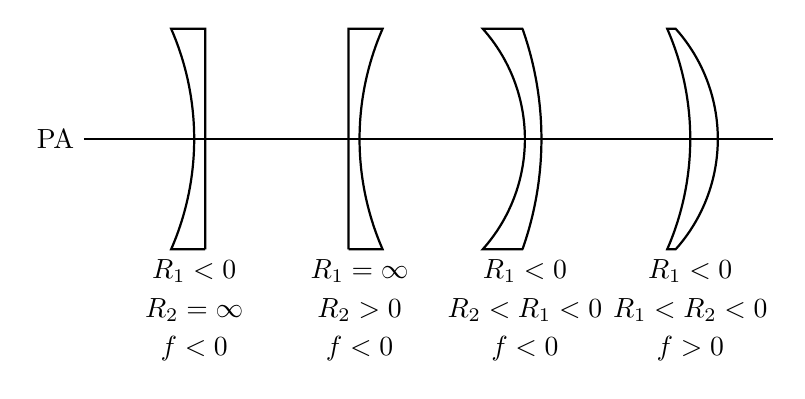
\begin{tikzpicture}[scale=.7,thick]
    \draw[thin] (-6,0)--(6.5,0) node[pos=0,left]{PA};
    
    \draw (-4,0) arc (0: asin(.4):5)--(-3.8, 2)--(-3.8,-2);
    \draw (-4,0) arc (0:-asin(.4):5)--(-3.8,-2);
    \node[below] at (-4,-2){$R_1<0$};
    \node[below] at (-4,-2.7){$R_2=\infty$};
    \node[below] at (-4,-3.4){$f<0$};
      
    \draw (-1,0) arc (180:180-asin(.4):5)--(-1.2, 2)--(-1.2,-2);
    \draw (-1,0) arc (180:180+asin(.4):5)--(-1.2,-2);
    \node[below] at (-1,-2){$R_1=\infty$};
    \node[below] at (-1,-2.7){$R_2>0$};
    \node[below] at (-1,-3.4){$f<0$};
      
    \draw (2,0) arc (0: asin(2/3):3)--(1.97, 2);
    \draw (2,0) arc (0:-asin(2/3):3)--(1.97,-2);
    \draw (2.3,0) arc (0: asin(1/3):6);
    \draw (2.3,0) arc (0:-asin(1/3):6);
    \node[below] at (2,-2){$R_1<0$};
    \node[below] at (2,-2.7){$R_2<R_1<0$};
    \node[below] at (2,-3.4){$f<0$};      
    \draw (5,0) arc (0: asin(.4):5)--(4.75, 2);
    \draw (5,0) arc (0:-asin(.4):5)--(4.75,-2);
    \draw (5.5,0) arc (0: asin(2/3):3);
    \draw (5.5,0) arc (0:-asin(2/3):3);
    \node[below] at (5,-2){$R_1<0$};
    \node[below] at (5,-2.7){$R_1<R_2<0$};
    \node[below] at (5,-3.4){$f>0$};      
  \end{tikzpicture}
\end{figure}

%
%
%
\subsection{Converging and Diverging Lenses}
When the focal length is positive (i.e.\ focal point is on the transmission
side, behind the lens), the lens is a \textbf{converging lens}:
\begin{figure}[ht]
  \centering
  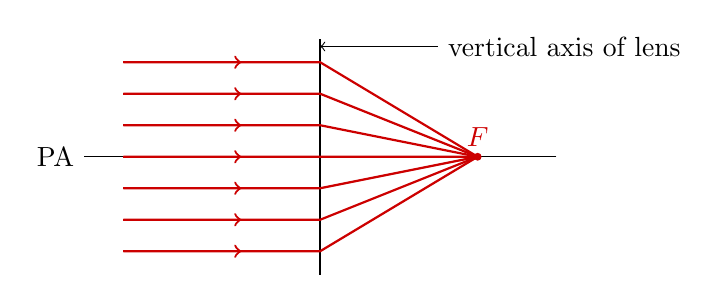
\begin{tikzpicture}
    \draw (3,0)--(-3,0) node[left]{PA};
    \draw[thick] (0,-1.5)--(0,1.5);
    \draw[<-] (0,1.4)--(1.5,1.4) node[right]{vertical axis of lens};
    \fill[red!80!black] (2,0) circle (.05) node[above]{$F$};
    \foreach \y in {-1.2,-.8,...,1.2}{
      \draw[red!80!black,thick] (-2.5,\y)--(0,\y)--(2,0);
      \draw[red!80!black,thick,->] (-2.5,\y)--(-1,\y);
    }
  \end{tikzpicture}
\end{figure}

%
%
%
%{Thin Lens Equation}
The \textbf{thin-lens equation} is exactly the same as the mirror equation:
\begin{equation}
  \boxed{\frac1s+\frac1{s'}=\frac1f}
\end{equation}
%  \begin{center}
%    \begin{tabular}{l|c|c}
%      \rowcolor{pink}
%      \textbf{Quantity} & \textbf{Symbol} & \textbf{SI Unit} \\ \hline
%      Distance to object & $s$  & \si\metre \\
%      Distance to image  & $s'$ & \si\metre \\
%      Focal length       & $f$  & \si\metre
%    \end{tabular}

\begin{center}
  \begin{tabular}{ccl}
    \hline
    $s$ & $+$ & real object: for objects in front of the lens (incident side) \\
    & $-$ & virtual object: for objects behind the lens (transmission side)\\
    \hline
    $s'$ & $+$ & real image: behind the lens (transmission side)\\
    & $-$ & virtual image: in front of the lens (incident side)\\
    \hline
  \end{tabular}
\end{center}

%{Lateral Magnification}
Likewise, the \textbf{lateral magnification} of the image is given by the
same equation as the mirror, but this time using the sign convention for
the thin lens:
\begin{equation}
  \boxed{
    m=\frac{h'}h=-\frac{s'}s
  }
\end{equation}

%    \begin{tabular}{l|c|c}
%      \rowcolor{pink}
%      \textbf{Quantity} & \textbf{Symbol} & \textbf{SI Unit} \\ \hline
%      Magnification factor & $m$ & (no units)\\
%      Object height & $h$  & \si\metre \\
%      Image height  & $h'$ & \si\metre \\
%      Distance to object & $s$  & \si\metre \\
%      Distance to image  & $s'$ & \si\metre
%    \end{tabular}
%  \end{center}

